\part{Laboratory Session 07}
\section{Introduction}
In this session everything was prepared to put the BalanBot into operation. Unfortunately all BalanBots were already borrowed when everything was ready.

\section{System Initialization}
First the MPU6050 has to be initialized.

	\begin{figure}[H]
		\centering
		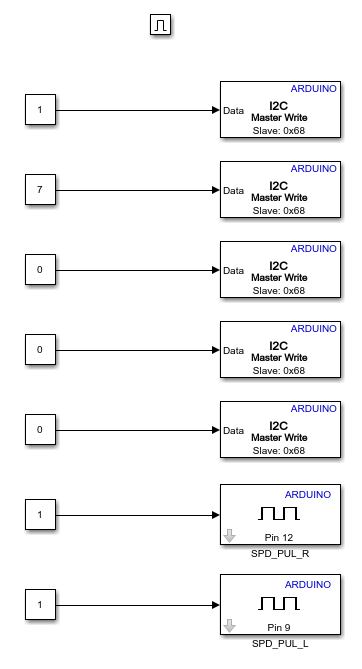
\includegraphics[width=0.25\textwidth]{figures/init.PNG}
		\caption{The initialization}	
		Source: Own presentation	
		\label{fig:init}	
	\end{figure}

	\begin{mdframed}
		\begin{lstlisting}[caption={C-Code from the script}, language=c,label={lst:init}]
	i2cData[0] = 7; // Set the sample rate to 1000Hz - 8kHz/(7+1) = 1000Hz
	i2cData[1] = 0x00; // Disable FSYNC and set 260 Hz Acc filtering, 256 Hz Gyro filtering, 8 KHz sampling
	i2cData[2] = 0x00; // Set Gyro Full Scale Range to +-250deg/s
	i2cData[3] = 0x00; // Set Accelerometer Full Scale Range to +-2g
	while (i2cWrite(0x19, i2cData, 4, false)); // Write to all four registers at once
	while (i2cWrite(0x6B, 0x01, true)); // PLL with X axis gyroscope reference and disable sleep mode		
		\end{lstlisting}
	\end{mdframed}
	

	\begin{mdframed}
		\begin{lstlisting}[caption={Automatic generated C-Code from the model}, language=c,label={lst:init_real}]
	/* Start for Enabled SubSystem: '<Root>/One_time_initialization' */
	/* Constant: '<S1>/Constant1' */
	framework_I2CWrite4_Start(&framework_DW.I2CWrite);
	
	/* Constant: '<S1>/Constant2' */
	framework_I2CWrite4_Start(&framework_DW.I2CWrite1);
	
	/* Constant: '<S1>/Constant3' */
	framework_I2CWrite4_Start(&framework_DW.I2CWrite2);
	
	/* Constant: '<S1>/Constant4' */
	framework_I2CWrite4_Start(&framework_DW.I2CWrite3);
	
	/* Start for MATLABSystem: '<S1>/I2C Write4' incorporates:
	*  Constant: '<S1>/Constant5'
	*/
	framework_I2CWrite4_Start(&framework_DW.I2CWrite4);
	
	/* Start for MATLABSystem: '<S6>/Digital Output' */
	framework_DW.obj_g.matlabCodegenIsDeleted = true;
	framework_DW.obj_g.isInitialized = 0;
	framework_DW.obj_g.matlabCodegenIsDeleted = false;
	framework_DW.objisempty_f = true;
	framework_DW.obj_g.isSetupComplete = false;
	framework_DW.obj_g.isInitialized = 1;
	digitalIOSetup(12, true);
	framework_DW.obj_g.isSetupComplete = true;
	
	/* Start for MATLABSystem: '<S5>/Digital Output' */
	framework_DW.obj_lq.matlabCodegenIsDeleted = true;
	framework_DW.obj_lq.isInitialized = 0;
	framework_DW.obj_lq.matlabCodegenIsDeleted = false;
	framework_DW.objisempty_e1 = true;
	framework_DW.obj_lq.isSetupComplete = false;
	framework_DW.obj_lq.isInitialized = 1;
	digitalIOSetup(9, true);
	framework_DW.obj_lq.isSetupComplete = true;
	
	/* End of Start for SubSystem: '<Root>/One_time_initialization' */	
	
	/* Terminate for Enabled SubSystem: '<Root>/One_time_initialization' */
	framework_I2CWrite4_Term(&framework_DW.I2CWrite);
	framework_I2CWrite4_Term(&framework_DW.I2CWrite1);
	framework_I2CWrite4_Term(&framework_DW.I2CWrite2);
	framework_I2CWrite4_Term(&framework_DW.I2CWrite3);
	
	/* Terminate for MATLABSystem: '<S1>/I2C Write4' */
	framework_I2CWrite4_Term(&framework_DW.I2CWrite4);
	
	/* Terminate for MATLABSystem: '<S6>/Digital Output' */
	matlabCodegenHandle_matlabCod_f(&framework_DW.obj_g);
	
	/* Terminate for MATLABSystem: '<S5>/Digital Output' */
	matlabCodegenHandle_matlabCod_f(&framework_DW.obj_lq);
	
	/* End of Terminate for SubSystem: '<Root>/One_time_initialization' */		
		\end{lstlisting}
	\end{mdframed}

	

\section{Read Gyro Sensor Data}
The sensor data is processed in this block. First they are converted into the data type int16. Then they are divided into angle and gyro.

	\begin{figure}[!htbp]
		\centering
		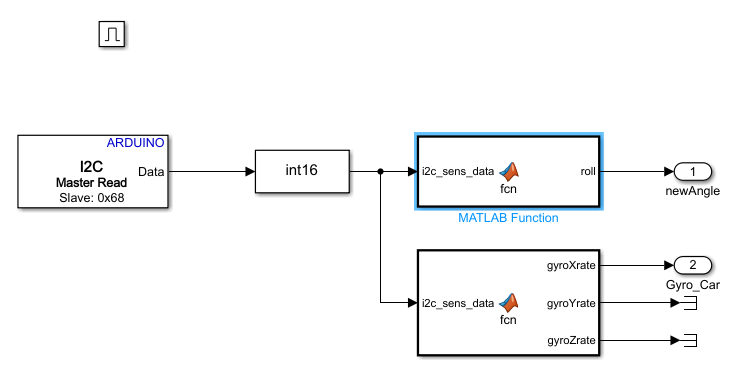
\includegraphics[width=0.3\textwidth]{figures/read.PNG}
		\caption{Processing of the read datas}	
		Source: Own presentation	
		\label{fig:read}	
	\end{figure}

	\begin{mdframed}
		\begin{lstlisting}[caption={Conversion from the acceleration to the angle}, language=matlab,label={lst:roll}]
	function roll = fcn(i2c_sens_data)
	accX = double(i2c_sens_data(1));
	accY = double(i2c_sens_data(2));
	accZ = double(i2c_sens_data(3));
	roll = atan(accY / sqrt(accX * accX + accZ * accZ)) * 180/pi;		
		\end{lstlisting}
	\end{mdframed}

	\begin{mdframed}
		\begin{lstlisting}[caption={Conversion to the gyros}, language=matlab,label={lst:gyro}]
	function [gyroXrate,gyroYrate,gyroZrate] = fcn(i2c_sens_data)
	gyroX = double(i2c_sens_data(5));
	gyroY = double(i2c_sens_data(6));
	gyroZ = double(i2c_sens_data(7));
	gyroXrate = gyroX/131;
	gyroYrate = gyroY/131;
	gyroZrate = gyroZ/131;	
		\end{lstlisting}
	\end{mdframed}


\section{Controller}

	\begin{figure}[!htbp]
		\centering
		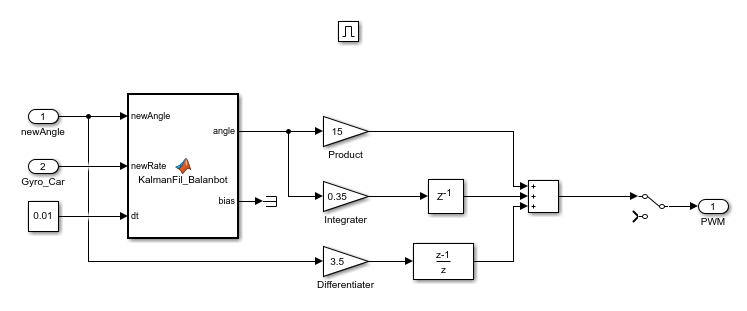
\includegraphics[width=0.7\textwidth]{figures/controller.PNG}
		\caption{....}	
		Source: Own presentation	
		\label{fig:controller}	
	\end{figure}


\section{Actuators}

	\begin{figure}[!htbp]
		\centering
		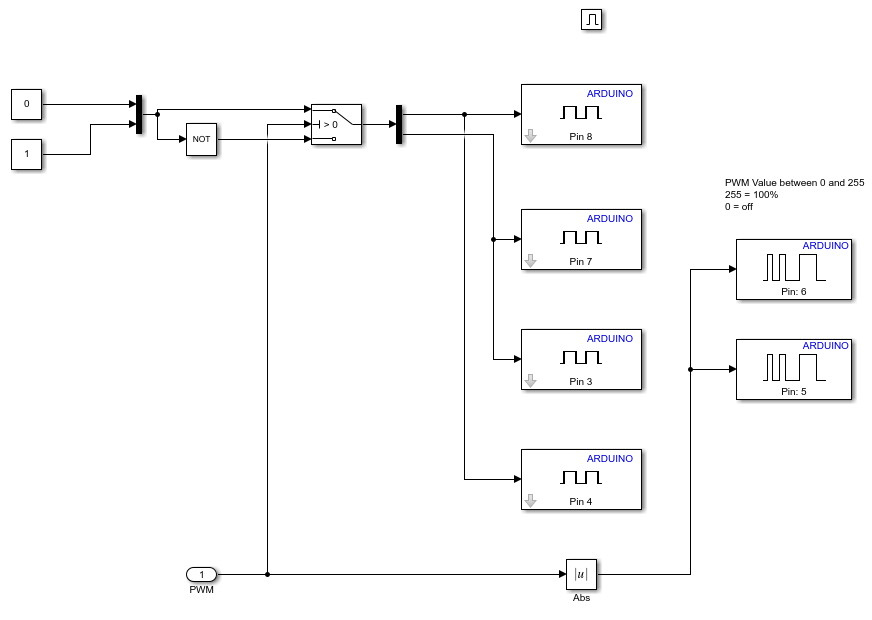
\includegraphics[width=0.7\textwidth]{figures/act.PNG}
		\caption{....}	
		Source: Own presentation	
		\label{fig:act}	
	\end{figure}


\section{Whole Structure}
Finally, all the blocks from the previous sections were assembled to form a single structure shown in Figure \ref{fig:struct}.

	\begin{figure}[!htbp]
		\centering
		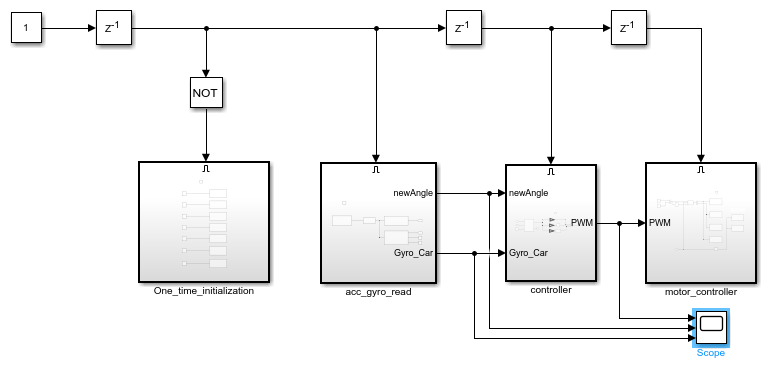
\includegraphics[width=0.7\textwidth]{figures/struct.PNG}
		\caption{The whole structure consist of blocks from the previous sections}	
		Source: Own presentation	
		\label{fig:struct}	
	\end{figure}




